\section*{Problem Statement} 
The objective of this problem is to solve a first-order differential equation numerically using the Gauss elimination method. The model describes exponential decay, governed by:
\[
\frac{dN}{dt} = -\lambda N, \quad N(0) = N_0,
\]
where $\lambda$ is the decay constant and $N_0$ is the initial value. The equation is discretized and solved as a linear system.

\section*{Methodology} 
The exponential decay equation is discretized using a finite-difference approximation:
\[
N_i - N_{i-1} = -\lambda \, t_{i-1} \, \Delta t, \quad i = 2,3,\ldots,N,
\]
with the initial condition $N_1 = N_0$.

This system can be written in matrix form:
\[
M \cdot \vec{N} = \vec{R},
\]
where $M$ is a lower bidiagonal matrix and $\vec{R}$ is the right-hand side vector incorporating the initial condition and decay terms.

The steps are:
\begin{enumerate}
  \item Construct matrix $M$ of size $N \times N$:
  \begin{itemize}
    \item $M(1,1) = 1$, 
    \item $M(i,i) = 1$, $M(i,i-1) = -1$ for $i \geq 2$.
  \end{itemize}
  \item Construct vector $\vec{R}$:
  \begin{itemize}
    \item $R(1) = N_0$, 
    \item $R(i) = -\lambda (i-1) \Delta t^2$ for $i \geq 2$.
  \end{itemize}
  \item Form augmented matrix $A = [M|\vec{R}]$.
  \item Apply Gaussian elimination to reduce $A$ to upper-triangular form.
  \item Use back-substitution to solve for $\vec{N}$.
\end{enumerate}

\subsection*{Pseudo-code}
\begin{enumerate}
  \item Define parameters: $\Delta t$, $t_{\max}$, $\lambda$, $N_0$.
  \item Construct $M$ and $\vec{R}$ as above.
  \item Form augmented matrix $A = [M|\vec{R}]$.
  \item Apply Gaussian elimination:
  \[
  A(r,:) = A(r,:) - \frac{A(r,p)}{A(p,p)} A(p,:), \quad r > p.
  \]
  \item Solve using back-substitution:
  \[
  N_p = \frac{A(p,n+1) - \sum_{j=p+1}^n A(p,j)N_j}{A(p,p)}.
  \]
  \item Plot $N(t)$ against time.
\end{enumerate}

\section*{Results} 
The given problem parameters are:
\[
\Delta t = 0.01, \quad t_{\max} = 5, \quad \lambda = 0.3, \quad N_0 = 100.
\]

The solution vector $\vec{N}$ was obtained numerically using Gaussian elimination. The figure below shows the computed decay curve:

\begin{figure}[h!]
  \centering
  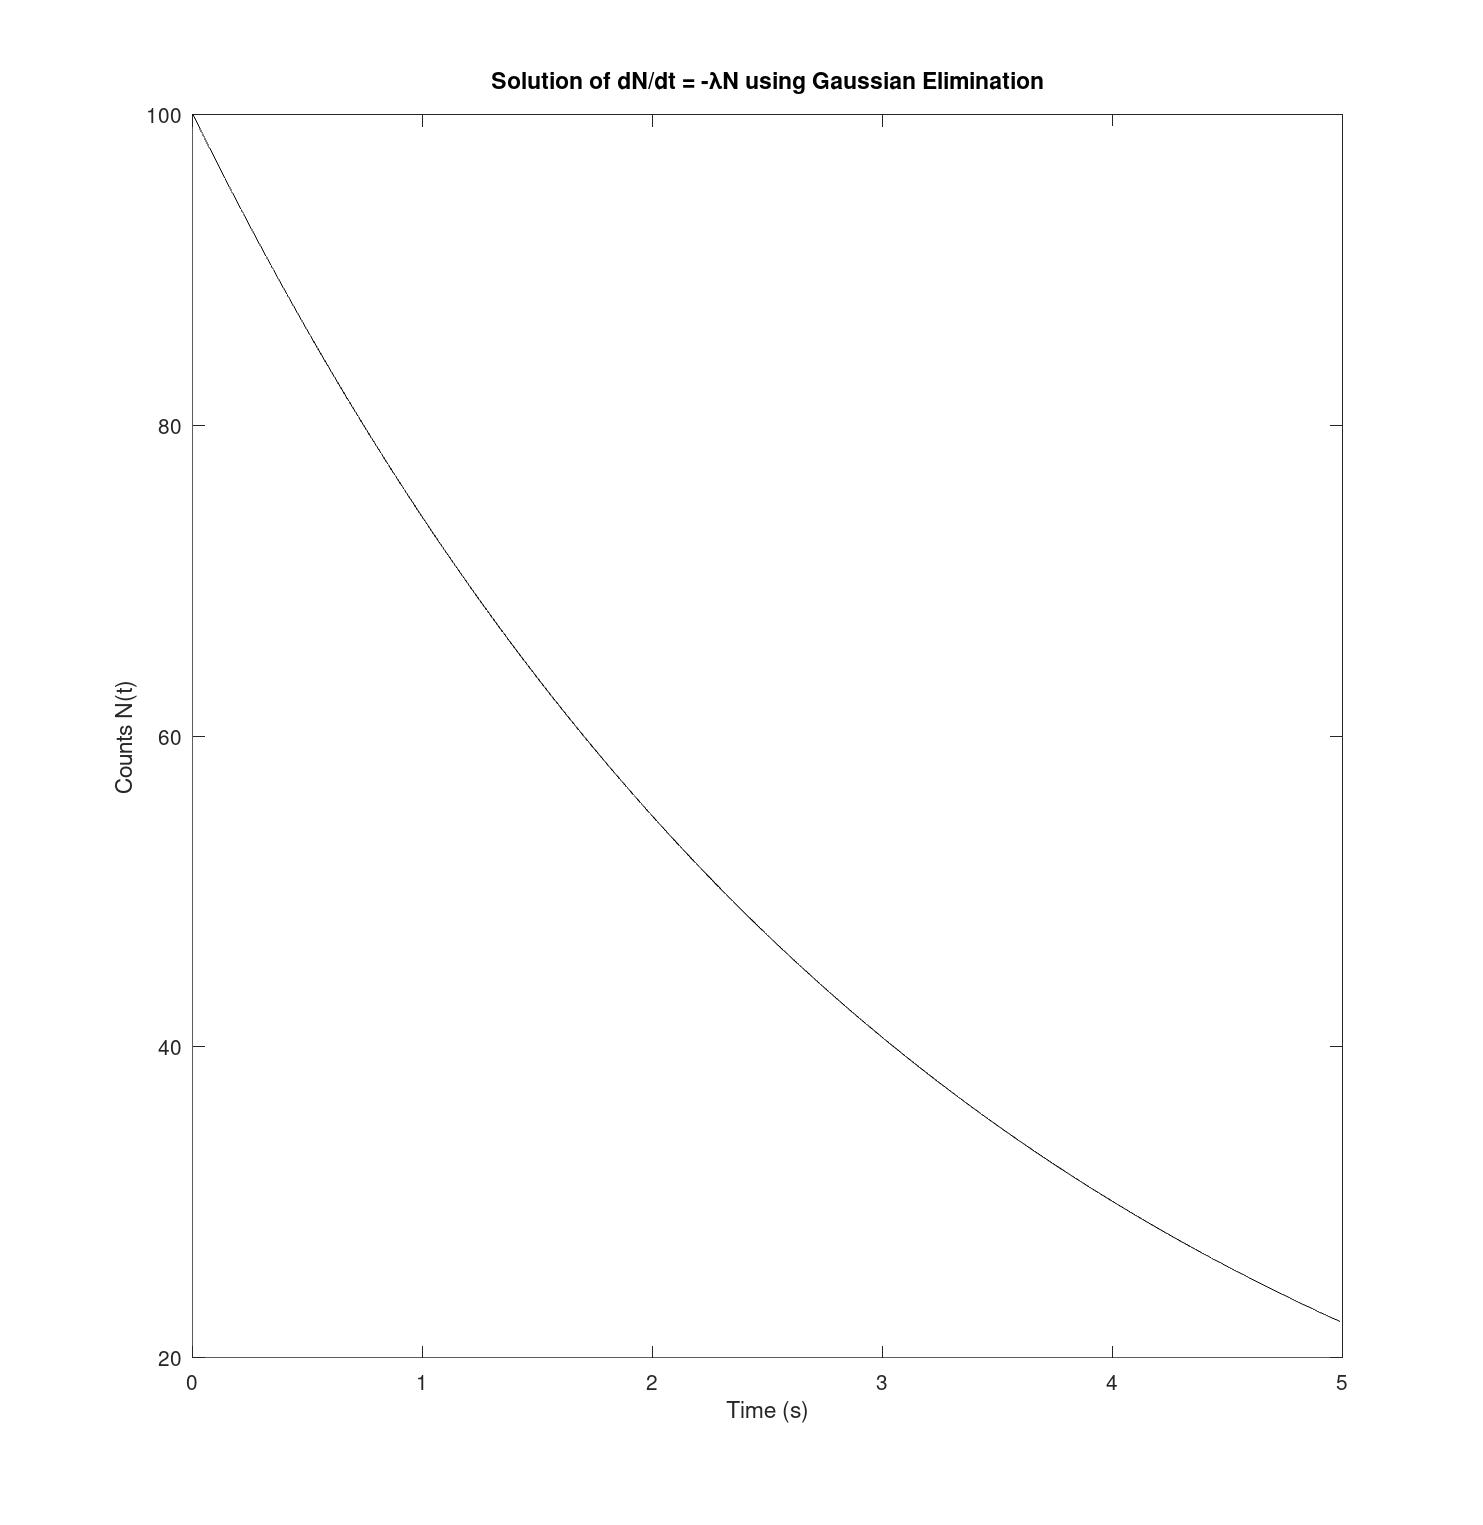
\includegraphics[width=0.8\textwidth]{a4.jpg}
  \caption{Numerical solution of $\tfrac{dN}{dt} = -\lambda N$ using Gaussian elimination}
  \label{fig:decay}
\end{figure}

The numerical solution matches the expected exponential decay behavior, decreasing monotonically from $N(0) = 100$.

\section*{Conclusion} 
The Gauss elimination method was successfully applied to solve the discretized form of a first-order decay differential equation. The computed results reproduce the exponential decay curve accurately. This demonstrates the viability of solving differential equations by converting them into linear systems and applying linear algebra techniques.

